\documentclass[12pt, a4paper]{article}

\usepackage[margin=2.5cm, headheight=15pt]{geometry}
\usepackage{booktabs}
\usepackage{tabularx}
\usepackage{array}
\usepackage{xcolor}
\usepackage{titlesec}
\usepackage{parskip}
\usepackage{hyperref}
\usepackage{enumitem}
\usepackage{fancyhdr}
\usepackage{colortbl}
\usepackage[T1]{fontenc}
\usepackage{lmodern}
\usepackage{tikz}
\usetikzlibrary{positioning}
\usepackage{tcolorbox}
\tcbuselibrary{skins, breakable, listings}
\usepackage{listings}
\usepackage{mdframed}
\usepackage{graphicx}

% -------------------------------------------------------------------------
% Colors
% -------------------------------------------------------------------------
\definecolor{pollityblue}{RGB}{0, 84, 166}
\definecolor{pollitylightblue}{RGB}{220, 235, 252}
\definecolor{okgreen}{RGB}{0, 120, 0}
\definecolor{lightgreen}{RGB}{220, 245, 220}
\definecolor{warnred}{RGB}{166, 0, 0}
\definecolor{lightred}{RGB}{252, 220, 220}
\definecolor{warnorange}{RGB}{200, 100, 0}
\definecolor{lightorange}{RGB}{255, 240, 220}
\definecolor{midgray}{RGB}{180, 180, 180}
\definecolor{codebg}{RGB}{245, 245, 245}
\definecolor{darkgray}{RGB}{60, 60, 60}

% -------------------------------------------------------------------------
% Section formatting
% -------------------------------------------------------------------------
\titleformat{\section}{\large\bfseries\color{pollityblue}}{}{0em}{}[\titlerule]
\titleformat{\subsection}{\normalsize\bfseries\color{darkgray}}{}{0em}{\thesubsection\quad}
\renewcommand{\thesubsection}{\arabic{subsection}}

% -------------------------------------------------------------------------
% Header / Footer
% -------------------------------------------------------------------------
\pagestyle{fancy}
\fancyhf{}
\fancyhead[L]{\small\textit{Pollity --- \$1,000 Bootstrap MVP Plan}}
\fancyhead[R]{\small\textit{Internal / Confidential}}
\fancyfoot[C]{\thepage}
\renewcommand{\headrulewidth}{0.4pt}

% -------------------------------------------------------------------------
% Hyperref
% -------------------------------------------------------------------------
\hypersetup{
    colorlinks=true,
    linkcolor=pollityblue,
    urlcolor=pollityblue,
    pdftitle={Pollity \$1000 MVP Plan},
    pdfauthor={Piyush Zaware}
}

% -------------------------------------------------------------------------
% Custom boxes
% -------------------------------------------------------------------------
\newtcolorbox{insightbox}[1]{
    colback=#1!8!white,
    colframe=#1,
    boxrule=1.2pt,
    arc=4pt,
    left=8pt, right=8pt, top=5pt, bottom=5pt,
    breakable
}

\newtcblisting{treebox}{
    colback=codebg,
    colframe=midgray,
    boxrule=0.5pt,
    arc=2pt,
    left=8pt, right=8pt, top=6pt, bottom=6pt,
    listing only,
    listing options={
        basicstyle=\ttfamily\footnotesize,
        breaklines=true,
        columns=fullflexible,
        keepspaces=true
    },
    breakable
}

% -------------------------------------------------------------------------
\begin{document}

% =========================================================================
% TITLE PAGE
% =========================================================================
\begin{titlepage}
    \centering
    \vspace*{1.5cm}

    {\color{pollityblue}\rule{\linewidth}{2pt}}\\[0.4cm]
    {\Huge\bfseries\color{pollityblue} POLLITY}\\[0.3cm]
    {\large\itshape Building India's Last Mile of Digital Governance}\\[0.2cm]
    {\color{pollityblue}\rule{\linewidth}{2pt}}\\[1.2cm]

    {\LARGE\bfseries Bootstrap MVP Plan}\\[0.4cm]
    {\Large\color{warnred}\bfseries \$1,000 Constraint}\\[0.4cm]
    {\large Jan-Sunwai: Zero-to-Beta on a Shoestring}\\[1.2cm]

    \begin{tabular}{ll}
        \textbf{Budget:}          & \$1,000 total (hard ceiling) \\[0.3em]
        \textbf{Builder:}         & Piyush Zaware (CTO) --- solo engineering \\[0.3em]
        \textbf{Date:}            & March 2026 \\[0.3em]
        \textbf{Beta Goal:}       & 50 active users, NPS $>$ 40 \\[0.3em]
        \textbf{Monthly Burn:}    & \$10--15/month (infrastructure only) \\[0.3em]
        \textbf{Runway:}          & 60--80 months at infrastructure burn rate \\
    \end{tabular}

    \vspace{1.5cm}

    \begin{tcolorbox}[
        colback=lightred,
        colframe=warnred,
        boxrule=1.5pt,
        arc=4pt,
        title={\bfseries\color{warnred} Constraint Reframe},
        fonttitle=\bfseries
    ]
    \$1,000 is not a funding problem. \textbf{It is a prioritisation problem.}
    The technology to build Jan-Sunwai costs almost nothing --- Supabase, Vercel,
    Railway, and Anthropic's Claude Haiku API together cost under \$15/month.
    The real constraints are \textbf{Piyush's time} and \textbf{getting 50 representatives
    to actually use the product.} Reserve \$800+ for user acquisition,
    not infrastructure.
    \end{tcolorbox}

    \vfill
    {\color{midgray}\rule{0.5\linewidth}{0.5pt}}\\[0.3cm]
    {\small pollity.in \quad $\cdot$ \quad hello@pollity.in \quad $\cdot$ \quad \textcopyright\ 2026 Pollity}
\end{titlepage}

\tableofcontents
\newpage

% =========================================================================
% SECTION 1: WHAT CHANGES AT $1,000
% =========================================================================
\section{What Changes at \$1,000}

\begin{insightbox}{warnred}
\textbf{Original plan assumed \$55K for product development.}
At \$1,000, three things become non-negotiable:
\begin{itemize}[leftmargin=1.2em, itemsep=0.1em]
    \item No contractors. Piyush builds the entire stack.
    \item No AWS. Replace with managed free-tier platforms.
    \item No compliance/security spend until seed round.
\end{itemize}
Everything else stays the same. The product scope, the user target, the beta milestones --- unchanged.
\end{insightbox}

\vspace{0.8em}

\begin{table}[ht]
\centering
\caption{Original Plan vs. \$1,000 Bootstrap Plan}
\renewcommand{\arraystretch}{1.4}
\begin{tabularx}{\textwidth}{X p{3.5cm} p{3.5cm}}
\toprule
\rowcolor{pollitylightblue}
\textbf{Dimension} & \textbf{Original (\$100K)} & \textbf{Bootstrap (\$1,000)} \\
\midrule
Infrastructure         & AWS Mumbai (ap-south-1), \$12K/yr & Supabase + Vercel + Railway, \$10--15/mo \\
Backend hosting        & ECS Fargate + ALB                 & Railway (\$5/mo, always-on) \\
Database               & RDS Postgres + managed backups    & Supabase free tier (500MB, daily backups) \\
Frontend hosting       & AWS S3 + CloudFront               & Vercel free tier \\
Redis / Queue          & ElastiCache (\$50+/mo)            & Upstash Redis free tier (10K/day) \\
NLP                    & Claude API + fine-tuning budget   & Claude Haiku API (\$0.25/1M tokens) \\
Contractors            & \$28K (6-week sprint)             & None --- CTO builds solo \\
Security audit         & \$4,600                           & Deferred to seed round \\
DPDP compliance setup  & \$3K legal                        & Deferred to seed round \\
ISO 27001 assessment   & Part of \$15K ops budget          & Deferred to seed round \\
Terraform / IaC        & Full AWS infrastructure code      & Platform UIs (no Terraform needed) \\
Docker (local dev)     & Required for dev parity           & Optional --- run locally with \texttt{venv} \\
\midrule
\rowcolor{lightgreen}
\textbf{Monthly burn} & \$3,000--5,000 & \textbf{\$10--15} \\
\rowcolor{lightgreen}
\textbf{Runway}       & 20 months (at \$100K)  & \textbf{60--80 months} \\
\bottomrule
\end{tabularx}
\end{table}

\vspace{0.8em}

\begin{insightbox}{okgreen}
\textbf{The counterintuitive truth:} The \$1,000 plan has \textit{longer runway} than the \$100K plan
because the \$100K plan burns on salaries and AWS. Infrastructure is essentially free in 2026
if you use the right platforms. The bottleneck is never money at this stage --- it is
\textbf{time to ship} and \textbf{trust with political users}.
\end{insightbox}

\newpage

% =========================================================================
% SECTION 2: REVISED TECH STACK
% =========================================================================
\section{Revised Tech Stack: Zero-Cost Where Possible}

\subsection{Stack Overview}

\begin{table}[ht]
\centering
\caption{Bootstrap Tech Stack with Monthly Costs}
\renewcommand{\arraystretch}{1.5}
\begin{tabularx}{\textwidth}{>{\bfseries}p{2.5cm} p{3.5cm} X p{1.8cm}}
\toprule
\rowcolor{pollitylightblue}
\textbf{Layer} & \textbf{Service} & \textbf{Free Tier / Notes} & \textbf{Monthly Cost} \\
\midrule
Backend        & FastAPI on Railway      & 512MB RAM, always-on at \$5/mo Starter plan & \$5 \\
Frontend       & Next.js on Vercel       & Unlimited personal projects, 100GB bandwidth & \$0 \\
Database       & Supabase (free tier)    & 500MB Postgres, 50K MAU auth, Row Level Security & \$0 \\
Redis / Queue  & Upstash Redis           & 10,000 commands/day free --- enough for 50 beta users & \$0 \\
WhatsApp       & Meta Business API       & First 1,000 conversations/month free & \$0 \\
NLP            & Anthropic Claude Haiku  & \$0.25/1M input tokens. 50 users $\times$ 50 grievances = $\sim$\$0.10 total & $\sim$\$2--5 \\
Auth           & Supabase Auth           & Included in free tier & \$0 \\
File storage   & Supabase Storage        & 1GB included in free tier & \$0 \\
CI/CD          & GitHub Actions          & 2,000 min/month free & \$0 \\
Error tracking & Sentry free tier        & 5K errors/month, 14-day retention & \$0 \\
Analytics      & PostHog free tier       & 1M events/month, session recording & \$0 \\
Email (digest) & Resend free tier        & 3,000 emails/month free & \$0 \\
Domain         & pollity.in              & One-time annual renewal & \$15/yr \\
\midrule
\rowcolor{lightgreen}
\multicolumn{3}{l}{\textbf{Total monthly infrastructure cost}} & \textbf{\$7--10} \\
\bottomrule
\end{tabularx}
\end{table}

\subsection{Why These Specific Choices}

\textbf{Railway over Render (free tier):}
Render's free tier spins down the server after 15 minutes of inactivity. A WhatsApp webhook that arrives during a cold start will time out and Meta will stop sending webhooks. Railway's \$5/month Starter keeps the FastAPI process alive 24/7. This is non-negotiable for webhook reliability.

\textbf{Supabase over self-hosted Postgres:}
Supabase free tier gives you managed Postgres, Row Level Security (multi-tenant data isolation), built-in auth, realtime subscriptions, and daily backups --- for \$0. The equivalent on AWS would cost \$30--50/month minimum.

\textbf{Upstash Redis over Redis Cloud:}
Upstash charges per-request, not per-instance. 10,000 commands/day free is 300,000 commands/month --- more than sufficient for a 50-user beta processing hundreds of grievances. Redis Cloud free tier has connection limits that become problematic.

\textbf{Claude Haiku over GPT-4o-mini:}
Claude Haiku costs \$0.25/1M input tokens. For 50 beta users generating 50 grievances each, with average 200 tokens per classification request: 50 $\times$ 50 $\times$ 200 = 500,000 tokens = \textbf{\$0.13 total for the entire beta.} NLP is effectively free at this scale.

\textbf{No Terraform / no Docker required:}
At this scale (1 Railway service, 1 Vercel project, 1 Supabase project), infrastructure-as-code adds complexity without benefit. Platform UIs are sufficient. Docker can be added later when onboarding contractors.

\newpage

% =========================================================================
% SECTION 3: BUDGET ALLOCATION
% =========================================================================
\section{The \$1,000 Budget: Full Allocation}

\begin{insightbox}{pollityblue}
The most important insight in this document: \textbf{infrastructure costs \$7--10/month.}
That is \$120 for a full year. The remaining \$880 should not go to technology.
It should go to getting 50 representatives to actually use the product.
No amount of engineering solves a user acquisition problem.
\end{insightbox}

\vspace{0.8em}

\begin{table}[ht]
\centering
\caption{Full \$1,000 Budget Allocation}
\renewcommand{\arraystretch}{1.5}
\begin{tabularx}{\textwidth}{X p{2cm} X}
\toprule
\rowcolor{pollitylightblue}
\textbf{Category} & \textbf{Budget} & \textbf{What It Buys} \\
\midrule
\textbf{Infrastructure (12 months)}  & \$120  & Railway \$5/mo $\times$ 12 + Anthropic credits + domain renewal \\
\midrule
\textbf{User Acquisition}            & \$600  & Train tickets Delhi/Mumbai, coffee meetings with MLAs and councillors, 2--3 field trips to constituency offices, printing of onboarding guides in Hindi \\
\midrule
\textbf{WhatsApp Business Setup}     & \$50   & Meta Business verification, test message volume during development \\
\midrule
\textbf{Contingency}                 & \$230  & Unexpected API overages, extra travel, emergency tooling \\
\midrule
\rowcolor{lightgreen}
\textbf{Total}                       & \textbf{\$1,000} & \\
\bottomrule
\end{tabularx}
\end{table}

\vspace{1em}

\subsection{What Gets Deferred (and Why It Is Fine)}

\begin{table}[ht]
\centering
\caption{Deferred Items and When to Revisit}
\renewcommand{\arraystretch}{1.4}
\begin{tabularx}{\textwidth}{X p{2.5cm} X}
\toprule
\rowcolor{pollitylightblue}
\textbf{Deferred Item} & \textbf{Revisit When} & \textbf{Why It Is Fine to Defer} \\
\midrule
AWS Mumbai migration (DPDP)      & Seed round (\$300K+) & DPDP enforcement rules are not yet final. No regulator will target a 50-user pre-seed startup. Migrate before commercial launch. \\
ISO 27001 assessment             & Series A             & Required for enterprise/government contracts, not for beta. \\
Penetration test / security audit & Seed round          & With 50 beta users, attack surface is minimal. Basic OWASP checklist is sufficient. \\
Contractor engineering support   & Seed round           & CTO can build the full Jan-Sunwai v1 solo in 14--16 weeks. \\
Docker / Terraform / IaC         & When first contractor joins & Adds 2 weeks of setup time with zero user-facing benefit. \\
Multi-language NLP fine-tuning   & After beta data collected & Need real grievance data first. Generic Claude Haiku handles Hindi/Marathi adequately for beta. \\
\bottomrule
\end{tabularx}
\end{table}

\newpage

% =========================================================================
% SECTION 4: SIMPLIFIED ARCHITECTURE
% =========================================================================
\section{Simplified Architecture for Bootstrap}

At \$1,000, the architecture removes every layer that is not essential for the core user flow.

\subsection{System Diagram}

\begin{center}
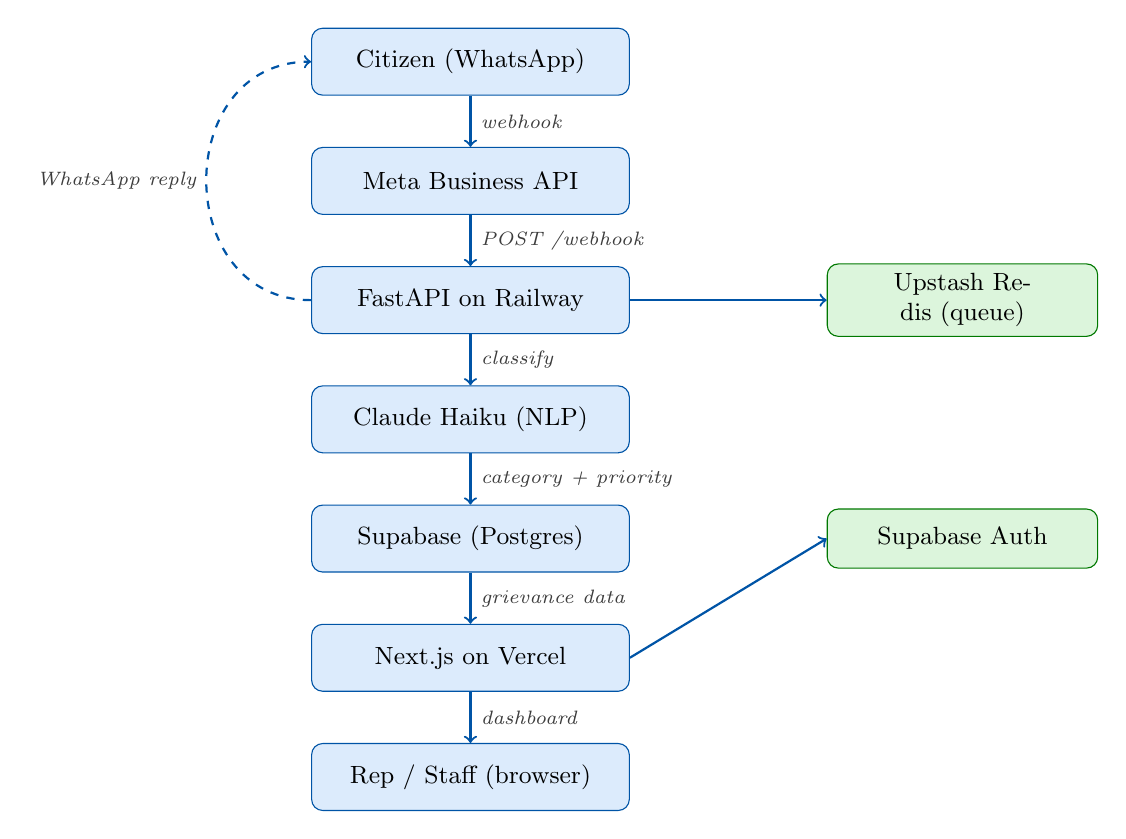
\begin{tikzpicture}[
    node distance=0.65cm and 2.5cm,
    box/.style={rectangle, rounded corners=4pt, draw=pollityblue, fill=pollitylightblue,
                text width=3.8cm, align=center, minimum height=0.85cm, font=\small},
    service/.style={rectangle, rounded corners=4pt, draw=okgreen, fill=lightgreen,
                    text width=3.2cm, align=center, minimum height=0.75cm, font=\small},
    arrow/.style={->, thick, color=pollityblue},
    label/.style={font=\scriptsize\itshape, color=darkgray}
]
    % Main flow (left column)
    \node[box] (citizen)   {Citizen (WhatsApp)};
    \node[box, below=of citizen] (meta)    {Meta Business API};
    \node[box, below=of meta]    (railway) {FastAPI on Railway};
    \node[box, below=of railway] (haiku)   {Claude Haiku (NLP)};
    \node[box, below=of haiku]   (supabase){Supabase (Postgres)};
    \node[box, below=of supabase](vercel)  {Next.js on Vercel};
    \node[box, below=of vercel]  (staff)   {Rep / Staff (browser)};

    % Side services
    \node[service, right=of railway] (upstash) {Upstash Redis (queue)};
    \node[service, right=of supabase] (auth)   {Supabase Auth};

    % Arrows
    \draw[arrow] (citizen)   -- node[label, right]{webhook} (meta);
    \draw[arrow] (meta)      -- node[label, right]{POST /webhook} (railway);
    \draw[arrow] (railway)   -- node[label, right]{classify} (haiku);
    \draw[arrow] (haiku)     -- node[label, right]{category + priority} (supabase);
    \draw[arrow] (supabase)  -- node[label, right]{grievance data} (vercel);
    \draw[arrow] (vercel)    -- node[label, right]{dashboard} (staff);
    \draw[arrow] (railway.east) -- (upstash.west);
    \draw[arrow] (vercel.east)  -- (auth.west);

    % Return arrow
    \draw[arrow, dashed] (railway.west) to[out=180, in=180, looseness=1.5]
        node[label, left]{WhatsApp reply} (citizen.west);
\end{tikzpicture}
\end{center}

\vspace{0.5em}

\subsection{What Is Removed vs. Original Architecture}

\begin{table}[ht]
\centering
\renewcommand{\arraystretch}{1.3}
\begin{tabularx}{\textwidth}{X p{1.8cm} X}
\toprule
\rowcolor{pollitylightblue}
\textbf{Component} & \textbf{Status} & \textbf{Replacement} \\
\midrule
AWS ECS / EC2              & Removed & Railway (\$5/mo) \\
AWS RDS                    & Removed & Supabase free Postgres \\
AWS ElastiCache            & Removed & Upstash free Redis \\
AWS CloudFront + S3        & Removed & Vercel free CDN \\
Terraform / IaC            & Removed & Platform UIs \\
Docker (local dev)         & Optional & Local Python venv + Supabase local CLI \\
Separate worker service    & Simplified & Background tasks handled within FastAPI using \texttt{BackgroundTasks} \\
Full CI/CD deploy pipeline & Simplified & GitHub Actions: test only; Railway auto-deploys from \texttt{main} branch \\
\bottomrule
\end{tabularx}
\end{table}

\newpage

% =========================================================================
% SECTION 5: REVISED FOLDER STRUCTURE
% =========================================================================
\section{Simplified Repository Structure}

At \$1,000 with a solo builder, complexity is the enemy. The repo structure is simplified to remove infrastructure-as-code, separate worker services, and multi-environment config.

\begin{treebox}
pollity-mvp/
|
+-- apps/
|   +-- web/                     # Next.js 14 frontend (Vercel)
|   |   +-- src/
|   |   |   +-- app/
|   |   |   |   +-- (auth)/      # login, register
|   |   |   |   +-- (dashboard)/ # main rep dashboard
|   |   |   |   |   +-- grievances/
|   |   |   |   |   +-- analytics/
|   |   |   |   |   +-- settings/
|   |   |   |   +-- onboarding/
|   |   |   +-- components/      # ui/, grievances/, layout/
|   |   |   +-- lib/             # api.ts, auth.ts, utils.ts
|   |   |   +-- types/           # grievance.ts, office.ts
|   |   +-- package.json
|   |   +-- next.config.js
|   |
|   +-- api/                     # FastAPI backend (Railway)
|       +-- app/
|       |   +-- main.py          # entry point
|       |   +-- core/
|       |   |   +-- config.py    # settings from env vars
|       |   |   +-- database.py  # Supabase + SQLAlchemy
|       |   +-- modules/
|       |   |   +-- jan_sunwai/
|       |   |   |   +-- router.py
|       |   |   |   +-- models.py
|       |   |   |   +-- schemas.py
|       |   |   |   +-- service.py
|       |   |   |   +-- whatsapp.py
|       |   |   +-- auth/
|       |   |   +-- offices/
|       |   +-- workers/
|       |       +-- classifier.py  # Claude Haiku pipeline
|       +-- tests/
|       +-- alembic/               # DB migrations
|       +-- requirements.txt
|
+-- docs/
|   +-- architecture.md
|   +-- onboarding.md            # new dev: running in 10 min
|   +-- data-model.md
|   +-- whatsapp-setup.md
|
+-- scripts/
|   +-- seed_db.py               # insert test grievances
|   +-- test_webhook.py          # simulate WhatsApp message
|
+-- .github/
|   +-- workflows/
|       +-- ci.yml               # lint + tests on every PR
|
+-- .env.example
+-- .gitignore
+-- README.md
\end{treebox}

\vspace{0.5em}

\begin{insightbox}{okgreen}
\textbf{What is removed from the original structure:}
\begin{itemize}[leftmargin=1.2em, itemsep=0.1em, topsep=0.2em]
    \item \texttt{infra/terraform/} --- no AWS, no Terraform needed
    \item \texttt{infra/docker-compose.yml} --- optional for solo dev
    \item \texttt{deploy.yml} --- Railway auto-deploys from \texttt{main} branch push
    \item Separate \texttt{workers/} service --- background tasks stay inside FastAPI
\end{itemize}
This is \textbf{not cutting corners}. It is right-sizing architecture for the current team size (1 person) and current user base (0 to 50 people).
\end{insightbox}

\newpage

% =========================================================================
% SECTION 6: BUILD TIMELINE
% =========================================================================
\section{Build Timeline: 14 Weeks Solo to Beta}

Piyush builds this alone. The timeline below is calibrated assuming 20--25 hours/week of coding time (evenings and weekends around academic responsibilities).

\begin{table}[ht]
\centering
\caption{14-Week Solo Build Timeline}
\renewcommand{\arraystretch}{1.6}
\begin{tabularx}{\textwidth}{p{2cm} p{3cm} X}
\toprule
\rowcolor{pollitylightblue}
\textbf{Weeks} & \textbf{Phase} & \textbf{Deliverables} \\
\midrule
1--2  & Foundation     & Supabase project setup + DB schema. Railway FastAPI skeleton. Vercel Next.js skeleton with auth. WhatsApp Business API application submitted to Meta. GitHub Actions CI. \texttt{.env.example} complete. \\
\midrule
3--5  & WhatsApp Core  & Webhook receiver with HMAC verification. Message parsed and queued via Upstash. Claude Haiku classification pipeline (language + category + priority). Grievance written to Supabase. Auto-acknowledgement sent to citizen. \\
\midrule
6--9  & Dashboard      & Rep dashboard: grievance list, filters (status/category/date), detail view. Status management (Open $\to$ In Progress $\to$ Resolved $\to$ Closed). Status change triggers WhatsApp notification to citizen. Staff invite + role system. Basic rep onboarding flow. \\
\midrule
10--11 & Polish        & Bulk actions. Analytics page (volume, resolution time, category breakdown). Mobile-responsive layout. Weekly email digest (Resend). CSV export. \\
\midrule
12--13 & Beta Prep     & Security basics (OWASP Top 10 self-audit, auth token review). DPDP-lite: data retention policy, consent message to citizens. In-app NPS via PostHog. Onboarding guide PDF in English + Hindi. Load test: simulate 200 concurrent messages. \\
\midrule
14    & Beta Launch    & Onboard first 10 representative offices in Delhi (personal network via Noorul). Monitor, fix bugs. Week 14 = real users, real grievances, real feedback. \\
\bottomrule
\end{tabularx}
\end{table}

\vspace{0.5em}

\subsection{Parallel Track: User Acquisition (Manav + Noorul)}

While Piyush builds, Manav and Noorul run the user pipeline. The product launches into a prepared audience, not into a void.

\begin{table}[ht]
\centering
\caption{14-Week User Acquisition Track}
\renewcommand{\arraystretch}{1.4}
\begin{tabularx}{\textwidth}{p{2cm} X}
\toprule
\rowcolor{pollitylightblue}
\textbf{Weeks} & \textbf{Activities} \\
\midrule
1--4   & Map personal network: list every MLA, councillor, and panchayat leader known directly or one degree away. Target: 20 warm contacts. \\
\midrule
5--8   & First meetings: coffee + demo of prototype (even basic). Collect pain points. Ask: ``Would you use a WhatsApp system that categorises and tracks grievances for you?'' Get verbal commitments. \\
\midrule
9--12  & Sign up 10 rep offices for beta. Get one staff member per office committed as the primary user. Collect their WhatsApp number for the business API. \\
\midrule
13--14 & Onboard beta users. Personally sit with each office for 1 hour. Show them the dashboard. Send first test grievance together. \\
\midrule
15+    & Expand to 50 offices. Weekly check-ins. Collect NPS. Document 5 case studies. \\
\bottomrule
\end{tabularx}
\end{table}

\newpage

% =========================================================================
% SECTION 7: THE HARD TRUTHS
% =========================================================================
\section{The Hard Truths at \$1,000}

\begin{insightbox}{warnred}
\textbf{Hard Truth 1: You cannot hire anyone.}
At \$1,000, there is no budget for contractors, freelancers, or part-time developers.
Piyush must build the entire stack: FastAPI backend, Next.js frontend, WhatsApp
integration, Claude API pipeline, Supabase schema, and deployment. This is achievable
in 14 weeks at 20--25 hours/week --- but only if scope is ruthlessly controlled.
Every feature request that is not Jan-Sunwai v1 must be rejected until beta.
\end{insightbox}

\vspace{0.5em}

\begin{insightbox}{warnred}
\textbf{Hard Truth 2: DPDP compliance is deferred.}
The original plan calls for India-based servers (AWS Mumbai) for DPDP Act compliance.
At \$1,000, the backend runs on Railway (US/EU servers). This is a legal grey area for
a pre-seed startup with 50 users. The pragmatic answer: DPDP enforcement rules are not
yet finalised, and no regulator will pursue a zero-revenue startup with 50 users.
Migrate to AWS Mumbai at the Seed round. \textbf{Document the decision and the plan to fix it.}
Do not pretend the risk does not exist --- acknowledge it in the beta user agreements.
\end{insightbox}

\vspace{0.5em}

\begin{insightbox}{warnred}
\textbf{Hard Truth 3: The biggest risk is not technical.}
The tech will work. Claude Haiku classifies Hindi grievances. WhatsApp webhooks are
reliable. Supabase handles the load. The existential risk is whether 50 elected
representatives will actually change their workflow to use a new tool --- even a free one.
Political users are resistant to change. Trust takes time. The \$600 in the user
acquisition budget is more important than the \$120 in infrastructure budget.
\end{insightbox}

\vspace{0.5em}

\begin{insightbox}{warnred}
\textbf{Hard Truth 4: The NPS target requires product quality, not features.}
NPS $>$ 40 from 50 political users means the product must be genuinely useful,
not just functional. This means: the WhatsApp auto-reply must be in the constituent's
language and sound human. The dashboard must load fast on a 4G mobile browser.
The classification must be accurate enough that the rep trusts it.
Speed and accuracy of these three things matter more than any additional feature.
\end{insightbox}

\newpage

% =========================================================================
% SECTION 8: WHAT TO BUILD FIRST
% =========================================================================
\section{Build Order: The Optimal Sequence}

At \$1,000 with one builder, sequencing matters. The wrong order wastes weeks on
infrastructure that breaks when the real bottleneck is elsewhere.

\begin{table}[ht]
\centering
\caption{Optimal Build Sequence with Rationale}
\renewcommand{\arraystretch}{1.5}
\begin{tabularx}{\textwidth}{>{\centering\bfseries}p{0.6cm} X p{3.5cm}}
\toprule
\rowcolor{pollitylightblue}
\textbf{\#} & \textbf{Build This} & \textbf{Why This Order} \\
\midrule
1 & Supabase schema: \texttt{offices}, \texttt{grievances}, \texttt{messages}, \texttt{staff} & Everything else depends on the data model. Get this right first --- changing it later is painful. \\
\midrule
2 & FastAPI webhook endpoint: receive Meta POST, verify HMAC signature, write raw message to \texttt{messages} table & This is the one piece that can break silently. Test it with real WhatsApp messages before building anything else on top. \\
\midrule
3 & Claude Haiku classifier: takes raw message, returns language + category + priority as JSON & This is the core AI value-add. Validate accuracy on 20--30 real Hindi/Marathi test messages before wiring it into the flow. \\
\midrule
4 & Auto-acknowledgement: send WhatsApp reply to citizen confirming receipt in their language & Validates the outbound API direction. Lets you demo a full loop (citizen sends $\to$ citizen gets reply) before the dashboard exists. \\
\midrule
5 & Supabase Auth + multi-tenant isolation: rep office login, RLS policies & Must exist before the dashboard. Do not skip RLS --- data isolation is a trust requirement, not a nice-to-have. \\
\midrule
6 & Next.js dashboard: grievance list + detail view + status update & First thing a rep actually sees. Polish this page above all others --- it determines NPS. \\
\midrule
7 & Status change $\to$ WhatsApp notification & Closes the loop for the citizen. This is the feature that makes representatives feel the system is working. \\
\midrule
8 & Analytics, bulk actions, email digest, CSV export & Usability improvements. Build these only after the core loop is validated with at least 5 real users. \\
\bottomrule
\end{tabularx}
\end{table}

\newpage

% =========================================================================
% SECTION 9: RISK REGISTER
% =========================================================================
\section{Bootstrap-Specific Risk Register}

\begin{table}[ht]
\centering
\caption{Risks Specific to the \$1,000 Bootstrap Scenario}
\renewcommand{\arraystretch}{1.5}
\begin{tabularx}{\textwidth}{X p{1.5cm} p{1.5cm} X}
\toprule
\rowcolor{pollitylightblue}
\textbf{Risk} & \textbf{Prob.} & \textbf{Impact} & \textbf{Mitigation} \\
\midrule
Piyush burns out or runs out of time & High & Critical & Enforce ruthless scope. Jan-Sunwai v1 only. If academic workload spikes, push beta by 4 weeks --- do not try to build faster. \\
Supabase free tier hits limits & Low & Medium & 500MB is ample for 50 beta users with 1,000 grievances. Monitor storage weekly. Upgrade to Pro (\$25/mo) only if hit. \\
Railway goes down mid-webhook & Low & High & Set up UptimeRobot (free) to ping the health endpoint every 5 min. WhatsApp retries failed webhooks for 7 days --- most messages will be recovered. \\
Meta rejects WhatsApp Business API & Medium & Critical & Apply immediately. Use Twilio WhatsApp sandbox as fallback for dev only. Have a backup plan: Telegram Bot API (same architecture, instant approval). \\
No one uses the product & High & Critical & The biggest risk. Mitigation: Noorul personally onboards the first 10 rep offices. Do not launch to cold contacts. \\
Claude Haiku misclassifies Hindi & Medium & Medium & Add human-review queue for confidence $<$ 0.7. In beta, low accuracy is a learning opportunity, not a failure. \\
Rep staff don't check dashboard & High & High & Make the WhatsApp flow standalone --- staff don't need to check the dashboard for the system to function. Dashboard is a bonus. \\
\bottomrule
\end{tabularx}
\end{table}

\newpage

% =========================================================================
% SECTION 10: UPGRADE PATH TO SEED
% =========================================================================
\section{The Upgrade Path: Bootstrap to Seed Round}

The \$1,000 bootstrap plan is not the destination --- it is the validation engine.
Once 50 users are active and NPS $>$ 40, the seed round (\$300--500K) is unlocked.
Here is exactly what changes when seed capital arrives.

\begin{table}[ht]
\centering
\caption{Bootstrap to Seed: What Gets Upgraded}
\renewcommand{\arraystretch}{1.4}
\begin{tabularx}{\textwidth}{X p{3.5cm} p{3.5cm}}
\toprule
\rowcolor{pollitylightblue}
\textbf{Component} & \textbf{Bootstrap (\$1K)} & \textbf{Post-Seed (\$300K+)} \\
\midrule
Backend hosting       & Railway \$5/mo                  & AWS ECS Fargate, ap-south-1 \\
Database              & Supabase free                   & AWS RDS Postgres, Mumbai \\
Data residency        & US/EU (Railway)                 & India (DPDP compliant) \\
Redis                 & Upstash free tier               & AWS ElastiCache \\
Infrastructure        & Platform UIs                    & Terraform IaC \\
Engineering           & CTO solo                        & 1 senior full-stack hire \\
NLP                   & Generic Claude Haiku            & Fine-tuned on beta grievance data \\
Security              & OWASP self-audit                & External pentest + ISO 27001 \\
Compliance            & Deferred                        & DPDP setup + legal counsel \\
\bottomrule
\end{tabularx}
\end{table}

\vspace{1em}

\begin{insightbox}{okgreen}
\textbf{The sequence that raises the seed round:}
\begin{enumerate}[leftmargin=1.5em, itemsep=0.2em]
    \item Ship Jan-Sunwai v1 on Railway + Supabase + Vercel.
    \item Onboard 50 representatives in Delhi and Maharashtra.
    \item Collect: NPS $>$ 40, 1,000+ grievances processed, 5 case studies, DAU/MAU $>$ 0.4.
    \item Show these numbers to investors.
    \item Raise \$300--500K seed.
    \item Migrate to AWS Mumbai, hire first engineer, begin Vidhayak-Mitra.
\end{enumerate}
\textbf{The bootstrap plan is not a compromise. It is the proof that the team can build
and ship without needing money --- which is the single most credible signal to a pre-seed investor.}
\end{insightbox}

\vfill
\begin{center}
    {\color{midgray}\rule{0.5\linewidth}{0.5pt}}\\[0.3cm]
    {\small\itshape Pollity --- Building India's Last Mile of Digital Governance}\\
    {\small pollity.in \quad $\cdot$ \quad hello@pollity.in \quad $\cdot$ \quad \textcopyright\ 2026 Pollity}
\end{center}

\end{document}
